%-----------------------------------------------------------------------------------------------------------------------------------------------%
%	The MIT License (MIT)
%
%	Copyright (c) 2021 Jitin Nair
%
%	Permission is hereby granted, free of charge, to any person obtaining a copy
%	of this software and associated documentation files (the "Software"), to deal
%	in the Software without restriction, including without limitation the rights
%	to use, copy, modify, merge, publish, distribute, sublicense, and/or sell
%	copies of the Software, and to permit persons to whom the Software is
%	furnished to do so, subject to the following conditions:
%	
%	THE SOFTWARE IS PROVIDED "AS IS", WITHOUT WARRANTY OF ANY KIND, EXPRESS OR
%	IMPLIED, INCLUDING BUT NOT LIMITED TO THE WARRANTIES OF MERCHANTABILITY,
%	FITNESS FOR A PARTICULAR PURPOSE AND NONINFRINGEMENT. IN NO EVENT SHALL THE
%	AUTHORS OR COPYRIGHT HOLDERS BE LIABLE FOR ANY CLAIM, DAMAGES OR OTHER
%	LIABILITY, WHETHER IN AN ACTION OF CONTRACT, TORT OR OTHERWISE, ARISING FROM,
%	OUT OF OR IN CONNECTION WITH THE SOFTWARE OR THE USE OR OTHER DEALINGS IN
%	THE SOFTWARE.
%	
%
%-----------------------------------------------------------------------------------------------------------------------------------------------%

%----------------------------------------------------------------------------------------
%	DOCUMENT DEFINITION
%----------------------------------------------------------------------------------------

% article class because we want to fully customize the page and not use a cv template

%%%% DEBUG COMMAND
%%%%\listfiles


%----------------------------------------------------------------------------------------
%	FONT
%----------------------------------------------------------------------------------------

% % fontspec allows you to use TTF/OTF fonts directly
% \usepackage{fontspec}
% \defaultfontfeatures{Ligatures=TeX}

% % modified for ShareLaTeX use
% \setmainfont[
% SmallCapsFont = Fontin-SmallCaps.otf,
% BoldFont = Fontin-Bold.otf,
% ItalicFont = Fontin-Italic.otf
% ]
% {Fontin.otf}

%----------------------------------------------------------------------------------------
%	PACKAGES
%----------------------------------------------------------------------------------------
\usepackage{url}
\usepackage{parskip} 	

%other packages for formatting
\RequirePackage{color}
\RequirePackage{graphicx}
\usepackage[usenames,dvipsnames]{xcolor}
\usepackage[scale=0.9]{geometry}

%tabularx environment
\usepackage{tabularx}

%for lists within experience section
\usepackage{enumitem}

% centered version of 'X' col. type
\newcolumntype{C}{>{\centering\arraybackslash}X} 

%to prevent spillover of tabular into next pages
\usepackage{supertabular}
\usepackage{tabularx}
\newlength{\fullcollw}
\setlength{\fullcollw}{0.47\textwidth}

%custom \section
\usepackage{titlesec}				
\usepackage{multicol}
\usepackage{multirow}

%CV Sections inspired by: 
%http://stefano.italians.nl/archives/26
\titleformat{\section}{\Large\scshape\raggedright}{}{0em}{}[\titlerule]
\titlespacing{\section}{0pt}{10pt}{10pt}

%\titleformat{\subsection}{}{}{}{}[\titlerule]
%\titlespacing{\subsection}{0pt}{10pt}{10pt}


%for publications
%\usepackage[style=authoryear,sorting=ynt, maxbibnames=2]{biblatex}
%\usepackage[style=authoryear,sorting=ydnt,maxbibnames=100]{biblatex}

\usepackage[%backend=biber,
        style=numeric,
        %        sorting=ydnt,
        sorting=ymdDnt,
        maxbibnames=100,
        defernumbers=true,
%        dateabbrev=false, % abbrev month display
        alldates=long]{biblatex}

% SORT BY YEAR, MONTH, DAY (decreasing)
\DeclareSortingTemplate{ymdDnt}{
  \sort{
    \field{presort}
  }
  \sort[final]{
    \field{sortkey}
  }
  \sort[direction=descending]{
    \field{sortyear}
    \field{year}
    \literal{9999}
  }
  \sort[direction=descending]{
    \field[padside=left,padwidth=2,padchar=0]{month}
    \literal{99}
  }
  \sort[direction=descending]{
    \field[padside=left,padwidth=2,padchar=0]{day}
    \literal{99}
  }
  \sort{
    \field{sortname}
    \field{author}
    \field{sorttitle}
    \field{title}
  }
  \sort{
    \field{sorttitle}
  }
  \sort[direction=descending]{
    \field[padside=left,padwidth=4,padchar=0]{volume}
    \literal{9999}
  }
}








\defbibheading{subbibliography}[\refname]{\subsection{#1}}
\setcounter{secnumdepth}{0}



%% \usepackage[
%%   style=publist,
%%   maxnames=11,
%%   plnumbering=local,
%%   marginyear=true,
%% ]{biblatex}



%Setup hyperref package, and colours for links
\usepackage[unicode, draft=false,pdfauthor={David Doukhan (INA)},pdftitle={CV David Doukhan},pdfkeywords={machine learning, speech analysis, gender studies, computer vision}]{hyperref}
\definecolor{linkcolour}{rgb}{0,0.2,0.6}
\hypersetup{colorlinks,breaklinks,urlcolor=linkcolour,linkcolor=linkcolour}

% replace full url with hyperlink and symbol
\DeclareFieldFormat{url}{\mkbibacro{URL}\addcolon\space\href{#1}{\faExternalLink*}}
\newcommand{\myurl}[1]{URL:~\href{#1}{\faExternalLink*}}


\addbibresource{david_doukhan_ina.bib}
\addbibresource{david_doukhan_older.bib}
\addbibresource{david_doukhan_itw.bib}
\addbibresource{david_doukhan_unpublished.bib}
\setlength\bibitemsep{1em}

%for social icons
\usepackage{fontawesome5}

%debug page outer frames
%\usepackage{showframe}



%%% MYFILTER

\defbibcheck{nokeyword}{%
\iffieldundef{keywords}{}{\skipentry}}


\usepackage{tikz} 


%%% JOB COMMANDS

\newenvironment{jobshort}[2]
    {
    \begin{tabularx}{\linewidth}{@{}l X r@{}}
    \textbf{#1} & \hfill &  #2 \\[3.75pt]
    \end{tabularx}
    }
    {
    }

\newenvironment{joblong}[2]
    {
    \begin{tabularx}{\linewidth}{@{}l X r@{}}
    \textbf{#1} & \hfill &  #2 \\[3.75pt]
    \end{tabularx}
    \begin{minipage}[t]{\linewidth}
    \begin{itemize}[nosep,after=\strut, leftmargin=1em, itemsep=3pt,label=--]
    }
    {
    \end{itemize}
    \end{minipage}    
    }


%----------------------------------------------------------------------------------------
%	BEGIN DOCUMENT
%----------------------------------------------------------------------------------------
\begin{document}

% non-numbered pages
%\pagestyle{empty} 



%----------------------------------------------------------------------------------------
%	TITLE
%----------------------------------------------------------------------------------------

% \begin{tabularx}{\linewidth}{ @{}X X@{} }
% \huge{Your Name}\vspace{2pt} & \hfill \emoji{incoming-envelope} email@email.com \\
% \raisebox{-0.05\height}\faGithub\ username \ | \
% \raisebox{-0.00\height}\faLinkedin\ username \ | \ \raisebox{-0.05\height}\faGlobe \ mysite.com  & \hfill \emoji{calling} number
% \end{tabularx}

\begin{tabularx}{\linewidth}{@{} C @{}}
\Huge{David Doukhan, Ph.D.} \\[7.5pt]
\href{https://github.com/DavidDoukhan}{\raisebox{-0.05\height}\faGithub\ DavidDoukhan} \ $|$ \
\href{https://www.researchgate.net/profile/David-Doukhan}{\raisebox{-0.05\height}\faResearchgate\ David-Doukhan} \ $|$ \ 
\href{https://linkedin.com/in/david-doukhan}{\raisebox{-0.05\height}\faLinkedin\ david-doukhan}
%\href{https://mysite.com}{\raisebox{-0.05\height}\faGlobe \ mysite.com} \ $|$ \

\href{https://twitter.com/doukhan_david}{\raisebox{-0.05\height}\faTwitter \ doukhan\_david} \ $|$ \ 
\href{mailto:david.doukhan@gmail.com}{\raisebox{-0.05\height}\faEnvelope \ david.doukhan@gmail.com} \ $|$ \ 
\href{tel:+33678789781}{\raisebox{-0.05\height}\faMobile \ +33.6.78.78.97.81} \\
\end{tabularx}

\begin{tikzpicture}[remember picture, overlay]
  \node [anchor=north east, inner ysep=15pt, inner xsep=30pt]  at (current page.north east)
     {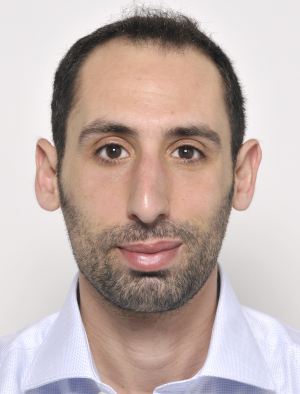
\includegraphics[height=3.2cm]{david_doukhan.jpg}};
\end{tikzpicture}

%\hfill
%\smash{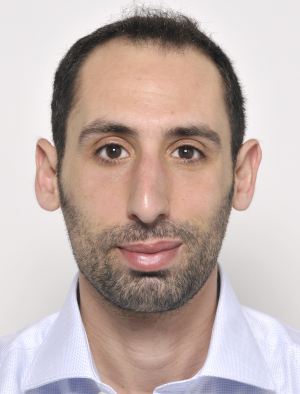
\includegraphics[width=2.5cm]{david_doukhan.jpg}}

%----------------------------------------------------------------------------------------
% EXPERIENCE SECTIONS
%----------------------------------------------------------------------------------------

%Interests/ Keywords/ Summary
\begin{en}
\section*{Summary}

I'm researcher at \href{https://www.ina.fr}{Institut National de l'Audiovisuel (INA)} in Paris metropolitan area (France).
This document presents some elements of my CV together with my detailed publication and research dissemination list (last update: \today).
More information to come!
%My research interest range from audio analysis and synthesis (audio segmentation, speaker diarization and recognition, paralinguistics, prosodic analysis 3D audio, speech synthesis), 
\end{en}

\begin{fr}
\section*{Résumé}

Je suis chercheur à l'\href{https://www.ina.fr}{Institut National de l'Audiovisuel (INA)} en région parisienne.
Ce document contient quelques éléments de mon CV, ainsi que la liste exhaustive de mes publications et travaux de dissémination scientifique (dernière mise à jour : \today).
Plus d'informations à venir!
\end{fr}



\tableofcontents

%% Experience
\begin{en}
\section{Work Experience}



\begin{joblong}{Speech analysis research engineer at INA}{2016 - present}
\item Supervision of intern and Ph.D. students on various ML tasks : speech interruptions detection, active-learning, speaker recognition and diarization, audio segmentation, active speaker detection, audio jingle detection, face classification.
\item Large-scale digital humanities studies based on the analysis of millions of hours of audiovisual data
\item Technological transfer of research results to several governmental and NGO reports related to women representation in media (ARCOM, GMMP, Calvez)
\item Implementation of audiovisual analysis softwares : sound and visual event detection, speech segmentation, voice activity detection, face tracking and classification, TV text incrustations detection, assisted annotation prototypes
\end{joblong}


\begin{joblong}{Large scale Music Information Retrieval at IRCAM}{2014-2015}
\item Distributed RAM ML algorithms implementation in Matlab
\item Refactorization of IRCAM’s classification framework to allow distributed processing
\item Proposal of supervector based music genre and mood detection models
\end{joblong}



\begin{jobshort}{Speaker analysis at LIMSI-CNRS}{2013-2014}
Implementation of speaker diarization and Voice Activity Detection algorithms suited to noisy archives (ethnographic recordings) in Python.
\end{jobshort}



\begin{joblong}{Text-To-Speech at LIMSI-CNRS : Ph.D. Research}{2009-2013}
\item Production of annotated speech ressources, prosodic analyzes and prosodic visualization tools
\item Natural language processing (CRF, POS) and inter-annotator agreement analysis
\item Expressive speech synthesis and perceptual evaluation
\end{joblong}



\begin{jobshort}{Real-time signal processing internship at Voxler}{2009 (6 months)}
Real-time pitch and prosodic similarity estimation applied to video-games (Matlab, C++)
\end{jobshort}

\begin{jobshort}{Virtual reality engineer at IRCAM}{2008 (6 months)}
Virtual environments to treat dog phobia: computer graphics programming, 3D binaural sound rendering \& head-tracking management in C++
\end{jobshort}

\begin{jobshort}{Computer Vision research assistant at MIT (USA)}{2008 (6 months)}
Face and object recognition (Python)
\end{jobshort}

\begin{jobshort}{High-throughput deep learning internship at MIT(USA)}{2007 (6 months)}
Implementation of a CNN Python framework suited to Cell Be parallel architectures : C, assembly, SIMD, code generation, just-in-time compilation.
\end{jobshort}


\end{en}



%% %Projects
%% \section{Projects}

%% \begin{tabularx}{\linewidth}{ @{}l r@{} }
%% \textbf{Some Project} & \hfill \href{https://some-link.com}{Link to Demo} \\[3.75pt]
%% \multicolumn{2}{@{}X@{}}{long long line of blah blah that will wrap when the table fills the column width long long line of blah blah that will wrap when the table fills the column width long long line of blah blah that will wrap when the table fills the column width long long line of blah blah that will wrap when the table fills the column width}  \\
%% \end{tabularx}

%% %----------------------------------------------------------------------------------------
%% %	EDUCATION
%% %----------------------------------------------------------------------------------------


\begin{en}
\section{Education}
\begin{tabularx}{\linewidth}{@{}l X@{}}	
2009-2013 & Ph.D. in Computer Science under the supervision of Christophe D’Alessandro (LIMSI-CNRS) and Albert Rilliard (LIMSI-CNRS), Paris Sud University.\\
2008-2009 & Master of Sciences ATIAM (Acoustics, Signal Processing and Computer Sciences applied to Music) co-hosted by University Pierre et Marie Curie (Paris VI), IRCAM, and Telecom Paris.\\
2005 & Student Exchange Program in Indian Institute of Technology Kanpur (India). Validated courses: Indian Art And Civilization, Machine Learning, Signal Processing, Mathematics\\
2001-2007 & EPITA (School of Engineering and Computer Science), major Artificial Intelligence and Machine Learning (SCIA). Graduated with honours (mention bien)\\
2001 & Scientist Baccalaureat (A-level), major physic\\
\end{tabularx}
\end{en}


\begin{fr}
\section{Formation}
\begin{tabularx}{\linewidth}{@{}l X@{}}	
2009-2013 & Doctorat en Informatique sous la direction de Christophe D’Alessandro (LIMSI-CNRS) et Albert Rilliard (LIMSI-CNRS), Université Paris Sud.\\
2008-2009 & Master Recherche ATIAM (Acoustique, Traitement du signal et Informatique Appliqués à la Musique) co-tutelle UPMC (Paris VI), IRCAM et Telecom Paris.\\
2005 & \'Echange universitaire à l'Indian Institute of Technology Kanpur (Inde). Cours suivis: art et civilisation indienne, apprentissage automatique, traitement du signal, mathématiques\\
2001-2007 & EPITA (Ecole pour l'informatique et les techniques avancées), majeure Intelligence Artificielle et Apprentissage Automatique (SCIA). Mention bien\\
2001 & Baccalaureat Scientifique, option physique\\
\end{tabularx}
\end{fr}


\section{\EvalSec}
\subsection{\EvalJournal}
\begin{enumerate}[nosep, after=\strut, leftmargin=1em, itemsep=3pt]
\item European Association for Signal Processing (EURASIP) Journal on Audio, Speech, and Music Processing
\item The Journal of the Acoustical Society of America (JASA)
\item Frontiers in Computer Science
\item revue Traitement Automatique des Langues (TAL - ATALA)
\end{enumerate}
\subsection{\EvalConf}
\begin{enumerate}[nosep,after=\strut, leftmargin=1em, itemsep=3pt]
\item Annual Conference of the International Speech Communication Association (INTERSPEECH - ISCA)
\item International Conference on Acoustics, Speech, and Signal Processing (IEEE ICASSP)
\item International Conference on Language Resources and Evaluation (LREC)
\item Phonetics and Phonology in Europe (Pape)
\item Journées d’Etudes de la Parole (JEP - AFCP)
\end{enumerate}
\subsection{\EvalProj}

\begin{en}
\begin{enumerate}[nosep,after=\strut, leftmargin=1em, itemsep=3pt]
\item Member of International Federation of Television Archives (IFTA) Media Studies Grant Commission (2020-2021)
\item Member of French National Research Agency (ANR) CE38 evaluation committee (2018)
\end{enumerate}
\end{en}

\begin{fr}
\begin{enumerate}[nosep,after=\strut, leftmargin=1em, itemsep=3pt]
\item Membre de la commission d'attribution des bourses pour les études des médias de la Fédération Internationale des Archives de Télévision (FIAT/IFTA) (2020-2021)
\item Membre du comité d'évaluation CE38 (La Révolution numérique : rapports au savoir et à la culture) de l'Agence Nationale de la Recherche (ANR) (2018)
\end{enumerate}
\end{fr}

\subsection{\EvalAnim}
\begin{enumerate}[nosep,after=\strut, leftmargin=1em, itemsep=3pt]
\item Music Information Retrieval Evaluation eXchange (MIREX - 2018).
\begin{en}Task Captain in change of voice and music activity detection challenge in collaboration with\end{en}
\begin{fr}
Co-organisation du concours de détection de voix et de musique en collaboration avec
\end{fr}
Blai Meléndez-Catalán (BMAT/UPF) \myurl{https://www.music-ir.org/mirex/wiki/2018:Music_and/or_Speech_Detection}.
\item Journées d’étude et de Formation sur la Parole (JEFP - 2012).
\begin{en}Member of the organization committee \end{en}
\begin{fr}Membre du comité d'organisation \end{fr}
\end{enumerate}






%----------------------------------------------------------------------------------------
%	PUBLICATIONS
%----------------------------------------------------------------------------------------

\section{\PubSec}

\begin{refsection}[david_doukhan_ina.bib,david_doukhan_older.bib,david_doukhan_itw.bib,david_doukhan_unpublished]
\nocite{*}
\printbibliography[type=article, check=nokeyword, heading=subbibliography, title={\PubJournal}, resetnumbers=true]
\printbibliography[type=inproceedings, check=nokeyword, heading=subbibliography, title={\PubConf}, resetnumbers=true]
\printbibliography[type=inproceedings, keyword={abstract}, heading=subbibliography, title={\PubAbstract}, resetnumbers=true]
\printbibliography[type=thesis, heading=subbibliography, title={\PubPhd}, resetnumbers=true]


\section{\DiffSec}
\printbibliography[type=report, heading=subbibliography, title={\DiffContribRep}, resetnumbers=true]
\printbibliography[type=article, heading=subbibliography, keyword={general}, title={\DiffGeneral}, resetnumbers=true]
\printbibliography[type=inproceedings, keyword={invit}, heading=subbibliography, title={\DiffInvit}, resetnumbers=true]
\printbibliography[type=inproceedings, keyword={publicaudition}, heading=subbibliography, title={\DiffPublic}, resetnumbers=true]
\printbibliography[keyword={itw}, heading=subbibliography, title={\DiffItw}, resetnumbers=true]

\end{refsection}

%----------------------------------------------------------------------------------------
%	SKILLS
%----------------------------------------------------------------------------------------


%% \section{Skills}
%% \begin{tabularx}{\linewidth}{@{}l X@{}}
%% Some Skills &  \normalsize{This, That, Some of this and that etc.}\\
%% Some More Skills  &  \normalsize{Also some more of this, Some more that, And some of this and that etc.}\\  
%% \end{tabularx}

%% \vfill


\end{document}
